\documentclass[11pt,a4paper]{article}

% ---------------------------------------------------------------
% Welcome to FreedomTex! This example shows the most common LaTeX
% features. Press Ctrl+Enter (or the green Recompile button) to
% update the PDF on the right. Double-click anywhere in the PDF to
% jump to the matching line of code.
% ---------------------------------------------------------------

\usepackage[utf8]{inputenc}
\usepackage[T1]{fontenc}
\usepackage{lmodern}
\usepackage[margin=2.5cm]{geometry}
\usepackage{amsmath, amssymb}
\usepackage{graphicx}
\usepackage{booktabs}
\usepackage[numbers]{natbib}
\usepackage{xcolor}
\usepackage{hyperref}
\hypersetup{colorlinks=true, linkcolor=teal, citecolor=teal, urlcolor=blue}

\title{Getting Started with \LaTeX{} in FreedomTex}
\author{Your Name\\\small Multimedia University}
\date{\today}

\begin{document}

\maketitle

\begin{abstract}
This short document is a tour of \LaTeX. It shows how to structure a document with sections, write mathematics, include figures and tables, and cite references from a bibliography file.
\end{abstract}

\tableofcontents

\section{Introduction}
\label{sec:intro}

\LaTeX{} is a document preparation system used for theses, journal papers, reports and presentations. You write plain text with a few commands, and \LaTeX{} takes care of the layout. Text can be \textbf{bold}, \textit{italic}, \underline{underlined} or \texttt{monospaced}.

Paragraphs are separated by a blank line. You can refer to other parts of the document, such as Section~\ref{sec:maths}, and \LaTeX{} fills in the numbers for you.

\subsection{Lists}

Unordered lists use \texttt{itemize}:
\begin{itemize}
    \item Write your content.
    \item Let \LaTeX{} handle the formatting.
    \item Compile to see the result.
\end{itemize}

Numbered lists use \texttt{enumerate}:
\begin{enumerate}
    \item Create a project.
    \item Write and compile.
    \item Download the PDF.
\end{enumerate}

\section{Mathematics}
\label{sec:maths}

Inline maths goes between dollar signs, like $E = mc^2$ or $\alpha + \beta = \gamma$. Numbered equations use the \texttt{equation} environment:
\begin{equation}
    \int_{0}^{\infty} e^{-x^2} \, dx = \frac{\sqrt{\pi}}{2}.
    \label{eq:gauss}
\end{equation}
Equation~\eqref{eq:gauss} is the Gaussian integral. Several aligned equations:
\begin{align}
    f(x) &= (x + 1)^2 \\
         &= x^2 + 2x + 1.
\end{align}
A matrix and a sum:
\[
    A = \begin{pmatrix} 1 & 2 \\ 3 & 4 \end{pmatrix}, \qquad
    \sum_{k=1}^{n} k = \frac{n(n+1)}{2}.
\]

\section{Figures and Tables}

Figure~\ref{fig:chart} is an image stored in the \texttt{figures} folder of this project. Upload your own images with the upload button in the file tree.

\begin{figure}[htbp]
    \centering
    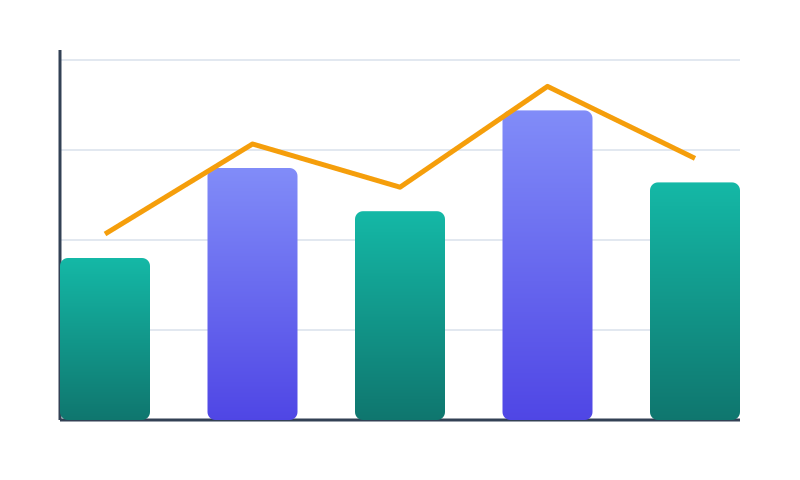
\includegraphics[width=0.6\textwidth]{figures/sample-chart.png}
    \caption{A sample chart included from the \texttt{figures} folder.}
    \label{fig:chart}
\end{figure}

Table~\ref{tab:results} uses the \texttt{booktabs} package for clean horizontal rules.

\begin{table}[htbp]
    \centering
    \caption{Example results.}
    \label{tab:results}
    \begin{tabular}{lcc}
        \toprule
        Method & Accuracy (\%) & Time (s) \\
        \midrule
        Baseline & 82.4 & 1.2 \\
        Proposed & \textbf{91.7} & 1.5 \\
        \bottomrule
    \end{tabular}
\end{table}

\section{Citations}

References live in \texttt{references.bib}. Cite them with \verb|\cite|, for example the classic \TeX{} book by \citet{knuth1984} or the \LaTeX{} manual \cite{lamport1994}. The bibliography below is built automatically.

\section{Conclusion}

You now know the basics. Explore the Insert and Format menus, try the Visual editor from the toolbar, and press F1 for a quick reference.

\bibliographystyle{plainnat}
\bibliography{references}

\end{document}
